\chapter{Introduccion}

En el presente trabajo práctico se abordará el análisis y la medición de parámetros eléctricos de diodos rectificadores y diodos zener. El objetivo principal es comprender el comportamiento de estos dispositivos en distintas condiciones de operación, tanto mediante el análisis teórico como a través de simulaciones y pruebas experimentales.

Se comenzará analizando circuitos propuestos por la cátedra, realizando cálculos de tensión, corriente y potencia. Luego, estos resultados serán validados mediante simulación, y finalmente se llevará a cabo la implementación física de los circuitos para tomar mediciones reales utilizando instrumentos como el multímetro y el osciloscopio.

Este práctico también servirá como repaso y afianzamiento de conceptos vistos en materias previas, permitiendo reforzar conocimientos fundamentales para futuras asignaturas de la carrera.

\section{Marco teorico}

El diodo es un componente electrónico que permite el paso de corriente en una sola dirección, bloqueando el flujo en sentido contrario. Esta propiedad lo convierte en un elemento fundamental para el proceso de rectificación, que consiste en convertir corriente alterna (CA) en corriente continua (CC).

El funcionamiento del diodo se basa en dos modos de polarización. En polarización directa, el diodo conduce corriente una vez superado cierto umbral de tensión (tensión de umbral). En cambio, en polarización inversa, impide el paso de corriente y se comporta como un circuito abierto.

La curva característica I-V del diodo refleja este comportamiento: en la región de polarización directa, la corriente aumenta rápidamente con una pequeña variación de tensión. En la región inversa, la corriente es prácticamente nula hasta alcanzar la tensión de ruptura, en la cual el diodo puede dañarse si no está diseñado para operar en esa condición.
Este comportamiento idealizado permite usar los diodos en múltiples aplicaciones, como rectificadores, protectores de polaridad y limitadores de tensión.

\begin{figure}[H]
  \centering
  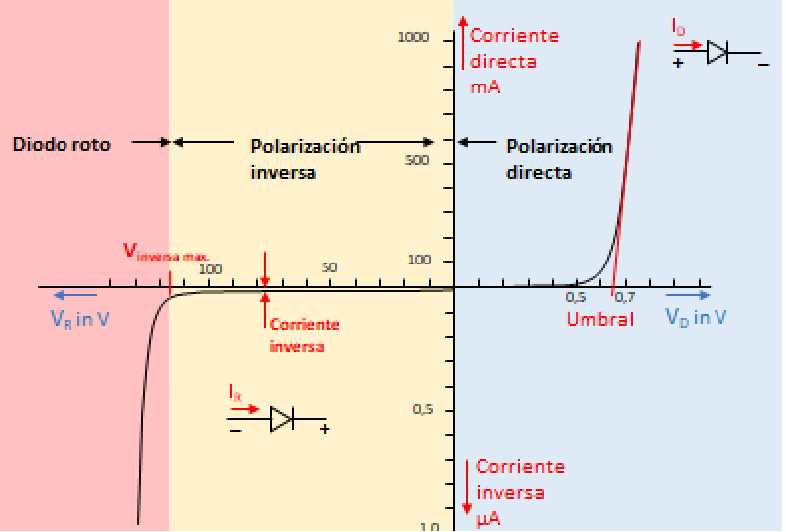
\includegraphics[width=0.60\textwidth]{images/diodos_rectificadores.png}
  \caption{Curva diodos rectificadores}
\end{figure}

El diodo Zener es un tipo especial de diodo semiconductor que, además de conducir en polarización directa como un diodo rectificador común, también está diseñado para operar en la región de ruptura cuando se encuentra polarizado en inversa. Esta característica lo convierte en una herramienta clave para la regulación de tensión.

A diferencia de los diodos rectificadores, los Zener permiten el paso de corriente en sentido inverso si la tensión aplicada supera un valor específico conocido como tensión Zener ($V_Z$). Esto es posible gracias a una unión P-N especialmente dopada, que permite que el dispositivo trabaje de forma segura y repetitiva en esa región sin dañarse.

El fenómeno de ruptura que permite este comportamiento puede ser de dos tipos: ruptura Zener, que predomina en dispositivos con $V_Z<6$, y ruptura por avalancha, que se manifiesta en Zeners con tensiones más elevadas. Ambos mecanismos están representados en la curva característica del dispositivo, donde se observa cómo el diodo, al alcanzar su tensión de ruptura en inversa, comienza a conducir fuertemente.

Gracias a esta propiedad, los diodos Zener son ampliamente utilizados en fuentes de alimentación y sistemas electrónicos como reguladores de tensión o protectores contra sobrevoltaje.

\begin{figure}[H]
  \centering
  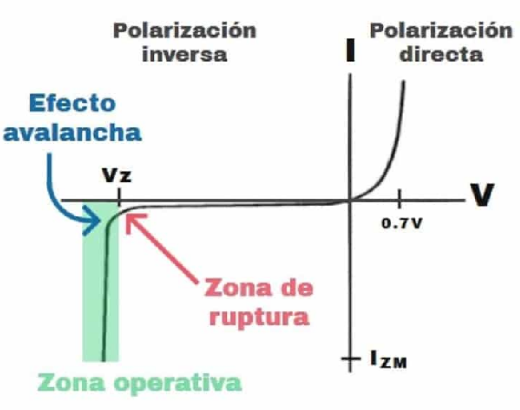
\includegraphics[width=0.60\textwidth]{images/diodos_zener.png}
  \caption{Curva diodos zener}
\end{figure}

\section{Encapsulados tipicos}

\begin{figure}[H]
  \centering
  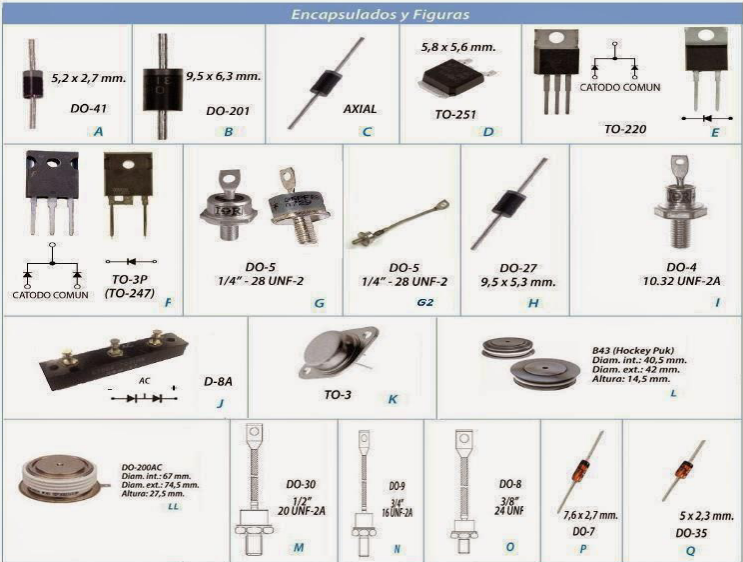
\includegraphics[width=0.50\textwidth]{images/encapsulados.png}
  \caption{Encapsulados comunes de diodos}
\end{figure}
